\documentclass[14pt, a4paper]{article}
\usepackage[T2A]{fontenc}
\usepackage[utf8]{inputenc}
\usepackage[russian]{babel}
\usepackage[left=3cm, right=1.5cm, top=2cm, bottom=2cm]{geometry}
\usepackage{indentfirst}
\usepackage{microtype}
\usepackage{array}
\usepackage{xcolor}
% \usepackage{times}
\usepackage{tempora}
\usepackage{ulem}
\usepackage{setspace}
\usepackage{amsmath}
\usepackage{booktabs}
\usepackage{graphicx}
\usepackage{float}
\usepackage{listings}
\graphicspath{{reports/figures/}{figures/}}
\lstset{basicstyle=\ttfamily\small, breaklines=true, columns=fullflexible, frame=single, keepspaces=true}
\pagestyle{empty}

\makeatletter
\renewcommand\section{\@startsection {section}{1}{\parindent}%
  {-3.5ex \@plus -1ex \@minus -.2ex}%
  {0.5ex}%
  {\normalfont\Large\bfseries}}
\renewcommand\tableofcontents{%
  \begin{center}\Large\bfseries\contentsname\end{center}%
  \@starttoc{toc}%
}
\renewcommand*\l@section{\@dottedtocline{1}{0em}{1.5em}}
\makeatother

\begin{document}
\onehalfspacing

\begin{center}
    \textbf{ФЕДЕРАЛЬНОЕ ГОСУДАРСТВЕННОЕ АВТОНОМНОЕ ОБРАЗОВАТЕЛЬНОЕ} \\
    \textbf{УЧРЕЖДЕНИЕ ВЫСШЕГО ОБРАЗОВАНИЯ} \\
    \textbf{«МОСКОВСКИЙ АВИАЦИОННЫЙ ИНСТИТУТ} \\
    \textbf{(НАЦИОНАЛЬНЫЙ ИССЛЕДОВАТЕЛЬСКИЙ УНИВЕРСИТЕТ)»}
\end{center}

\begin{center}
    \bfseries Институт №8 «Компьютерные науки и \\
    \bfseries прикладная математика» \\
    \bfseries Кафедра 806 «Вычислительная математика \\
    \bfseries и программирование»
\end{center}

\vspace{3cm}

\begin{center}
    \Large\bfseries Отчет \\
    \vspace{0.5cm}
    \mdseries по лабораторной работе №1.4
\end{center}

\vfill

\noindent
\hfill
\begin{tabular}{ll}
Группа:       & М8О-307Б-21 \\
Студент:      & М. С. Ивченко \\
Преподаватель:& доц. В. В. Киндинова \\
Оценка:       & \underline{\makebox[3cm][c]{}} \\ [0.2cm]
Дата:         & \underline{\makebox[3cm][c]{}}
\end{tabular}

\vfill

\begin{center}
    Москва \\
    2026
\end{center}

\newpage

\setcounter{tocdepth}{2}
\tableofcontents
\newpage

\section*{Тема}
\addcontentsline{toc}{section}{Тема}
Цель данной лабораторной работы -- изучить численный поиск собственных значений и собственных векторов симметрических матриц. В центре внимания находится метод вращений Якоби, который последовательно зануляет внедиагональные элементы и приводит матрицу к почти диагональному виду.

\section*{Задание}
\addcontentsline{toc}{section}{Задание}
Реализовать метод вращений в виде программы, задавая в качестве входных данных матрицу и точность вычислений. Используя разработанное программное обеспечение, найти собственные значения и собственные векторы симметрических матриц. Проанализировать зависимость погрешности вычислений от числа итераций.

\section*{Теория}
\addcontentsline{toc}{section}{Теория}
Метод вращений Якоби предназначен для нахождения собственных значений и собственных векторов вещественных симметрических матриц. Для таких матриц существует ортогональная матрица собственных векторов, а все собственные значения действительны. Метод строит последовательность ортогонально подобных матриц
\[
    A^{(k+1)} = U_k^T A^{(k)} U_k,
\]
поэтому собственные значения не меняются, но внедиагональные элементы постепенно уменьшаются.

На каждом шаге выбирается максимальный по модулю внедиагональный элемент $a_{ij}$. Затем строится матрица вращения $U_k$, которая отличается от единичной только в строках и столбцах $i$ и $j$. В плоскости этих координат она имеет элементы $\cos\varphi$ и $\sin\varphi$ и зануляет выбранный элемент $a_{ij}$.

Угол поворота вычисляется по формуле
\[
    \varphi = \frac12\arctan\frac{2a_{ij}}{a_{ii}-a_{jj}}.
\]
Если $a_{ii}=a_{jj}$, можно взять $\varphi=\pi/4$. После вращения сумма квадратов внедиагональных элементов уменьшается. Критерием остановки служит малая норма внедиагональной части:
\[
    \sqrt{\sum_{i<j} a_{ij}^2}<\varepsilon.
\]
Когда это условие выполнено, диагональные элементы текущей матрицы принимаются за собственные значения. Собственные векторы получаются как столбцы произведения всех матриц вращения:
\[
    V=U_1U_2\ldots U_k.
\]
Проверка результата выполняется подстановкой $Av_i\approx \lambda_i v_i$ и контролем ортогональности найденных векторов.

\begin{lstlisting}[language=Python]
index = _find_max_higher_diagonal(A)
phi = _calculate_phi(A, index)
A = _rotate(_rotate(A, phi, index).T, phi, index).T
eigen_vectors = _rotate(eigen_vectors, phi, index)
\end{lstlisting}

\section*{Ход лабораторной работы}
\addcontentsline{toc}{section}{Ход лабораторной работы}
Для матрицы
\[
A=\begin{pmatrix}
-3&-2&-4\\
-2&-3&-7\\
-4&-7&-3
\end{pmatrix}
\]
при $\varepsilon=10^{-5}$ метод завершился за 7 вращений. Найденные собственные значения:
\[
    \lambda_1=-1.30641125,\quad
    \lambda_2=-12.02290701,\quad
    \lambda_3=4.32931826.
\]
Максимальная проверочная невязка $\max |AV-V\Lambda|$ составила $5.25\cdot10^{-8}$.

\begin{figure}[H]
    \centering
    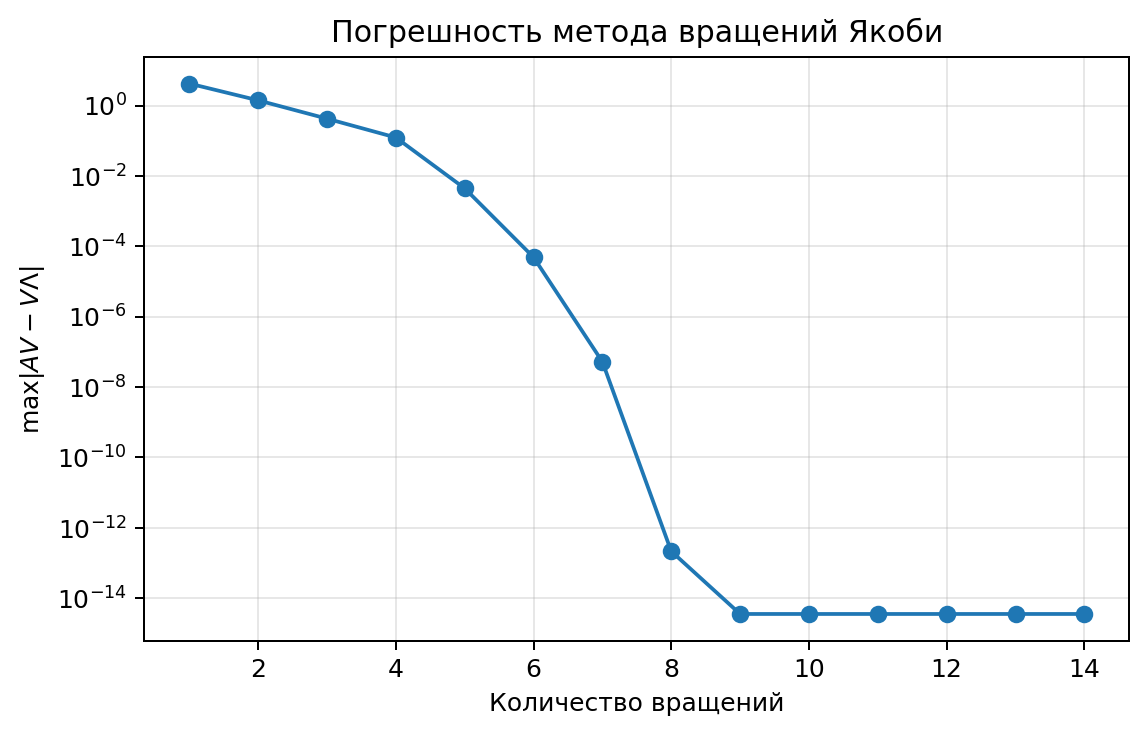
\includegraphics[width=0.86\textwidth]{lab1_4_jacobi_convergence.png}
    \caption{Проверочная погрешность метода Якоби при фиксированном числе вращений.}
\end{figure}

\section*{Выводы}
\addcontentsline{toc}{section}{Выводы}
Метод Якоби корректно нашел спектр симметрической матрицы и собственные векторы. После нескольких начальных шагов погрешность быстро уменьшается, а затем выходит на уровень машинного округления.

\end{document}
